\documentclass{article}
\usepackage{ctex}
\usepackage{authblk} 
\usepackage{indentfirst}
\usepackage{geometry}
\usepackage{listings}
\usepackage[usenames,dvipsnames]{xcolor}
\usepackage{appendix}
\usepackage{listings}
\usepackage{graphicx}
\usepackage{xcolor}
\usepackage{listings}
\setlength{\parindent}{2em} 
\lstset{
    basicstyle=\tt,
    keywordstyle=\color{purple}\bfseries,
    identifierstyle=\color{brown!80!black},
    commentstyle=\color{gray}
    showstringspaces=false,
}
\title{RECORD MANAGER 实验报告}
\author{张鑫\\3200102809@zju.edu.cn\\计算机科学与技术学院\\\date{}}


\begin{document}
\setlength{\parindent}{2em} 
\maketitle
\section[1]{绪论}
本次报告为浙江大学数据库系统课程夏学期大作业的RECORD MANAGER部分,由我个人完成,再这个模块的设计中,我完成了数据库Schema,Row,Coloum,Field的序列化操作,以及堆表的维护。
\section[2]{序列化}
\subsection[1]{序列化意义}
所谓序列化,即是将我们内存中对象转化为二进制的位流写入文件完成持久化操作,不同的对象有着不同的序列化规则。与之相对应的反序列化即是将文件中的二进制数据流读入内存生成对象。在本章中我们要完成数据库模式的序列化和反序列化。
序列化的具体实现实际上是向内存中一块buffer连续写入和读取,而将内存持久化则是底层模块的工作。
\subsection[2]{Scheme序列化}
任何对象序列化时都会先写入一个唯一的magic number用以标记该对象,在反序列化时能够起到校验作用。
由于scheme的私有成员是一个Column对象指针的Vector,因而要先写入vector的长度再顺序得将Vector中的Coloum进行序列化。
\subsection[3]{Row序列化}
Row是由rowid和一系列field构成的vector组成的,但与schema不同,Row不需要写入vector的size,这是由于我们可以根据以及反序列得到的schema对象得到field的长度。
Row只需要将vector中的field依次序列化即可,但需要注意,序列化每个域之前需要序列化is-null标志。
\subsection[4]{Column序列化}
coloum的序列化需要写入column的属性,值得注意的是诸如name这种字符串的序列化需要特殊处理。由于std::string的实际字符串存储在堆区,我们首先要序列化其长度,再将堆区的字符串实际存储拷贝到Buffer中。

\section[2]{堆表}
\subsection[1]{堆表页}
\begin{figure}
    \centering
    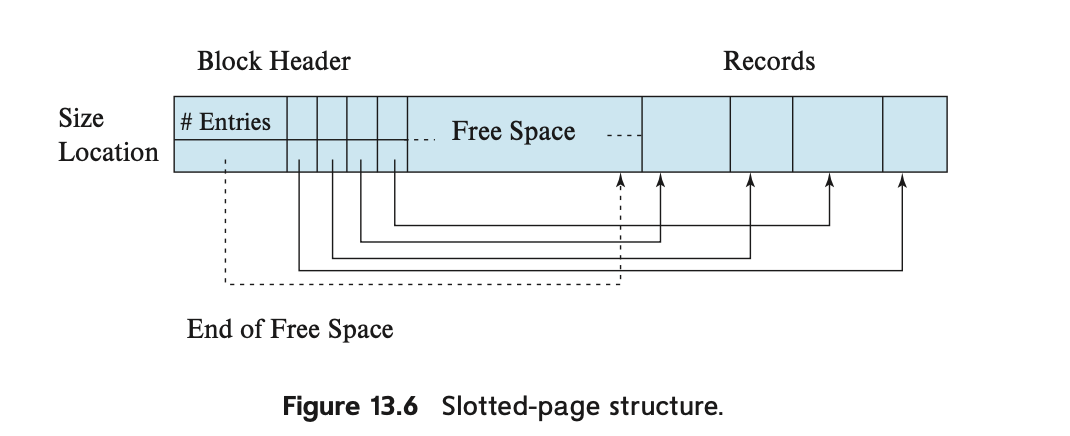
\includegraphics{picture/image.png}
\end{figure}

如图所示为堆表的一页,堆表就是由这样的页形成的双向链表构成的。
堆表页即TableHeapPage页由表头(Table Page Header)、空闲空间(Free Space)和已经插入的数据(Inserted Tuples)三部分组成。其中表头维护了PrevPageId、NextPageId、FreeSpacePointer以及每条记录在TablePage中的偏移和长度。插入的记录在页中从右向左扩展,每次插入记录时会将FreeSpacePointer的位置向左移动。
堆表页有自己的增删改方法,其中值得注意的是在堆表页中有MarkDelete和ApplyDelete两者删除方式,
其中,MarkDelete是一种lazy \ delete,是将要删除的Row的tuple \ size 置为无穷大,表示删除。\\
而ApplyDelete则是在物理上将tuple删除,并移动其他tuple使堆表页紧密排布。
update在堆表页中会有如下情景,若堆表页剩余空间较大,直接修改,若堆表页剩余空间没有修改后的tuple大,那么由上层模块将该tuple先删除再插入。

\subsection[2]{堆表}
堆表是存在与内存中而没有磁盘存储的对象,是堆表页的双向链表的manager,能够执行增删改查方法,并且带有迭代器。
\\ \indent
事实上堆表只需要维护堆表页的双向链表结构,通过调用底层模块的接口实现增上改查。
\\
值得注意的是堆表页的初始化,以及首次访问堆表头页需要进行初始化工作。
\\ \indent
本项目中的记录插入管理采用First \ Fit策略, 好处是堆表排布紧凑,缺点是需要以$O(N)$的时间找到可用的堆表页进行插入.
\subsection[3]{迭代器}
堆表迭代器结构定义如下:
\begin{lstlisting}
private:
  // add your own private member variables here
  Row* content;
  TableHeap* table_heap_;
  Transaction *txn_;
\end{lstlisting}

\indent 其中table\_heap\_*是只想堆表对象的指针,而Row*指向堆表中的tuple对象.迭代器的迭代原理实质上就是再堆表对象内部进行线性顺序访问的过程.本项目中以Row* \ content和TableHeao* \ table\_heap\_均为空指针为迭代器End().


\section[4]{测试结果}
\begin{figure}

    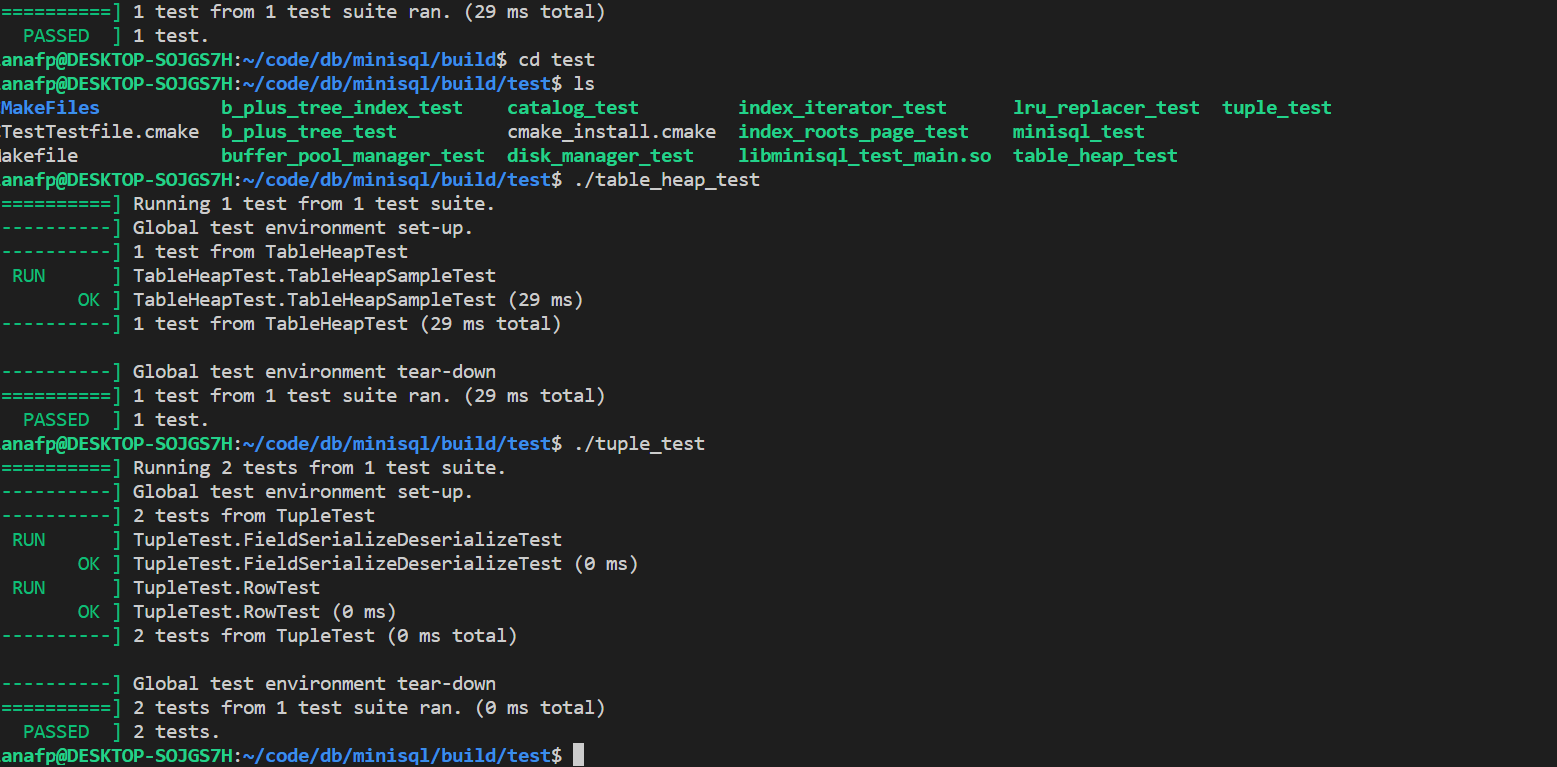
\includegraphics{picture/屏幕截图 2022-05-29 185052.png}
\end{figure}

\begin{appendices}
    \section[A]{序列化}
    \subsection[1]{schema}
    \begin{lstlisting}
        #include<iostream>
        using namespace std;
        #include "record/schema.h"

        uint32_t Schema::SerializeTo(char *buf) const {
          // replace with your code here
          uint32_t offset = 0;
          // write magic number
          MACH_WRITE_TO(uint32_t,buf+offset,Schema::SCHEMA_MAGIC_NUM);
          offset += sizeof(Schema::SCHEMA_MAGIC_NUM);
          // write columns count
          MACH_WRITE_TO(uint32_t,buf+offset,columns_.size());
          offset += sizeof(uint32_t);
          // write columns
          for(auto i:columns_){
            offset += i->SerializeTo(buf+offset);
          }
          return offset;
        }
        
        uint32_t Schema::GetSerializedSize() const {
          // replace with your code here
          uint32_t offset = sizeof(Schema::SCHEMA_MAGIC_NUM) + sizeof(uint32_t);
          for(auto i:columns_){
            offset += i->GetSerializedSize();
          }
          return offset;
        }
        
        uint32_t Schema::DeserializeFrom(char *buf, Schema *&schema, MemHeap *heap) {
          // replace with your code here
          // read magic num
          uint32_t offset = 0;
          uint32_t count = MACH_READ_UINT32(buf+offset);
          assert(count==Schema::SCHEMA_MAGIC_NUM);
        
          // create colums
          offset += sizeof(Schema::SCHEMA_MAGIC_NUM);
          std::vector<Column*> cols;
          // read count
          count = MACH_READ_UINT32(buf+offset);
          offset += sizeof(Schema::SCHEMA_MAGIC_NUM);
          cols.resize(count);
          for(uint32_t i=0;i<count;++i){
            offset += Column::DeserializeFrom(buf+offset,cols[i],heap);
          }
          // allocate schema
          schema = ALLOC_P(heap,Schema)(cols);
          return offset;
        }
        \end{lstlisting}
    \subsection[2]{row}
    \begin{lstlisting}
        #include "record/row.h"
        #include "glog/logging.h"
        #define ENABLE_BPM_DEBUG
        uint32_t Row::SerializeTo(char *buf, Schema *schema) const {
          // replace with your code here
          // assert(false);
          uint32_t offset = 0;
          // write row id
        
          // buf[0] = 16;
          
          MACH_WRITE_TO(RowId, buf + offset, rid_);
          // assert(false);
        
          offset += sizeof(RowId);
          // write fields
          uint32_t column_count = schema->GetColumnCount();
          uint32_t i = 0;
          // assert(false);
          for(i=0;i<column_count;i++)
          {
            MACH_WRITE_TO(bool,buf+offset,fields_[i]->IsNull());
            offset += sizeof(bool);
            offset += fields_[i]->SerializeTo(buf+offset);
          }
        
          return offset;
        }
        
        uint32_t Row::DeserializeFrom(char *buf, Schema *schema) {
          // replace with your code here
          // read row id
          uint32_t offset = 0;
          // read id
          this->rid_ = MACH_READ_FROM(RowId, buf + offset);
          offset += sizeof(RowId);
          // get column count
          uint32_t column_count = schema->GetColumnCount();
          if(column_count>fields_.capacity()) fields_.resize(column_count);
          for (uint32_t i = 0; i < column_count; ++i) {
            bool is_null = MACH_READ_FROM(bool,buf+offset);
            offset += sizeof(bool);
            if(is_null) continue;
            const Column *temp = schema->GetColumn(i);
            offset += this->fields_[i]->DeserializeFrom(buf + offset, temp->GetType(), &fields_[i],is_null,
            heap_);
          }
          return offset;
        }
        
        uint32_t Row::GetSerializedSize(Schema *schema) const {
          // replace with your code here
          uint32_t offset = 0;
          uint32_t colomn_count = schema->GetColumnCount();
          for (uint32_t i=0;i<colomn_count;++i) {
            offset += sizeof(bool);
            offset += this->fields_[i]->GetSerializedSize();
          }
          // if(offset==0) return 0;
          offset += sizeof(RowId);
          return offset;
        }
    \end{lstlisting}
    \subsection[3]{column}
    \begin{lstlisting}
        include "record/column.h"

Column::Column(std::string column_name, TypeId type, uint32_t index, bool nullable, bool unique)
        : name_(std::move(column_name)), type_(type), table_ind_(index),
          nullable_(nullable), unique_(unique) {
  ASSERT(type != TypeId::kTypeChar, "Wrong constructor for CHAR type.");
  switch (type) {
    case TypeId::kTypeInt :
      len_ = sizeof(int32_t);
      break;
    case TypeId::kTypeFloat :
      len_ = sizeof(float_t);
      break;
    default:
      ASSERT(false, "Unsupported column type.");
  }
}

Column::Column(std::string column_name, TypeId type, uint32_t length, uint32_t index, bool nullable, bool unique)
        : name_(std::move(column_name)), type_(type), len_(length),
          table_ind_(index), nullable_(nullable), unique_(unique) {
  ASSERT(type == TypeId::kTypeChar, "Wrong constructor for non-VARCHAR type.");
}

Column::Column(const Column *other) : name_(other->name_), type_(other->type_), len_(other->len_),
                                      table_ind_(other->table_ind_), nullable_(other->nullable_),
                                      unique_(other->unique_) {}

uint32_t Column::SerializeTo(char *buf) const {
  // replace with your code here
  // write magic num
  uint16_t offset = 0;
  MACH_WRITE_TO(uint32_t, buf + offset, COLUMN_MAGIC_NUM);
  offset += sizeof(COLUMN_MAGIC_NUM);
  // write name : string
  // write length of string
  uint32_t len = name_.length()+1;
  MACH_WRITE_TO(uint32_t, buf + offset, len);
  offset += sizeof(len);
  // addr
  char* addr = (char*)&name_[0];
  memcpy(buf+offset,addr,len);
  offset += len;
  // write type : TypeId
  MACH_WRITE_TO(TypeId, buf+offset, type_);
  offset += sizeof(TypeId);
  // write length
  MACH_WRITE_TO(uint32_t, buf+offset, len_);
  offset += sizeof(uint32_t);
  // write table index
  MACH_WRITE_TO(uint32_t, buf+offset, table_ind_);
  offset += sizeof(uint32_t);
  // write is_null_enable
  MACH_WRITE_TO(bool, buf+offset, nullable_);
  offset += sizeof(bool);
  // write is_uniqe
  MACH_WRITE_TO(bool, buf+offset, unique_);
  offset += sizeof(bool);
  return offset;
}

uint32_t Column::GetSerializedSize() const {
  // replace with your code here
  return sizeof(uint32_t) * 4 + sizeof(bool) * 2 + sizeof(TypeId) + 1 + name_.length();

}

uint32_t Column::DeserializeFrom(char *buf, Column* &column, MemHeap *heap) {
  // replace with your code here
  // read magic num
  uint16_t offset = 0;
  uint32_t r_magic_num = MACH_READ_FROM(uint32_t,buf+offset);
  if(r_magic_num!=Column::COLUMN_MAGIC_NUM){
#ifdef ENABLE_BPM_DEBUG
    log(ERROR)<<"The magic number not match when deserialize column!\n";
#endif
    return 0;
  }
  // magic number matched
  offset += sizeof(Column::COLUMN_MAGIC_NUM);
  // read name
  // read name length
  uint32_t name_len = MACH_READ_FROM(uint32_t,buf+offset);
  offset += sizeof(uint32_t);
  // read string
  std::string temp_str(buf + offset);
  offset += name_len;
  // read type
  TypeId temp_type = MACH_READ_FROM(TypeId,buf+offset);
  offset += sizeof(TypeId);
  // read length
  uint32_t temp_len = MACH_READ_FROM(uint32_t,buf+offset);
  offset += sizeof(uint32_t);
  // read table index 
  uint32_t temp_index = MACH_READ_FROM(uint32_t,buf+offset);
  offset += sizeof(uint32_t);
  // read null enable
  bool temp_nulleble = MACH_READ_FROM(bool,buf+offset);
  offset += sizeof(bool);
  // read unique
  bool temp_uniqe = MACH_READ_FROM(bool,buf+offset);
  offset += sizeof(bool);
  // consrtcut column
  if(temp_type==TypeId::kTypeChar)
  column = ALLOC_P(heap,Column)(temp_str,temp_type,temp_len,temp_index,temp_nulleble,temp_uniqe);
  else 
    column = ALLOC_P(heap,Column)(temp_str,temp_type,temp_index,temp_nulleble,temp_uniqe);
  return offset;
}

    \end{lstlisting}
    \section[B]{堆表}
    \begin{lstlisting}
        #include "storage/table_heap.h"
        #include "glog/logging.h"
        // #define ENABLE_BPM_DEBUG
        bool TableHeap::InsertTuple(Row &row, Transaction *txn) {
          // assert(row.GetSerializedSize()<PAGE_SIZE);
        
          page_id_t temp_page_id = this->first_page_id_;
          // assert(false);
          TablePage *table_page_ptr = reinterpret_cast<TablePage *>(buffer_pool_manager_->FetchPage(first_page_id_));
          assert(table_page_ptr!=nullptr);
          // search an availble table page
          if(table_page_ptr->GetPrevPageId()!=INVALID_PAGE_ID){
            table_page_ptr->Init(temp_page_id,INVALID_PAGE_ID,log_manager_,txn);
          }
          while (1) {
            // assert(false);
        #ifdef ENABLE_BPM_DEBUG
              LOG(INFO) << "page id: "<<temp_page_id<<"\n";
              LOG(INFO) << "page id: " <<table_page_ptr->GetPageId()<<"\n";
        #endif
            // try to insert
            if(table_page_ptr->InsertTuple(row,schema_,txn,lock_manager_,log_manager_)) break;
            // assert(false);
        #ifdef ENABLE_BPM_DEBUG
              LOG(INFO) <<"insert to this page false"<<"\n";
        #endif
            // check next page
            if (table_page_ptr->GetNextPageId() == INVALID_PAGE_ID) {
        #ifdef ENABLE_BPM_DEBUG
              LOG(INFO) << "NO AVAILABLE TABLE PAGE!\n";
        #endif
              // allocate new page
              page_id_t new_page_id;
              TablePage *new_page_ptr = reinterpret_cast<TablePage*>(buffer_pool_manager_->NewPage(new_page_id));
              // assert(new_page_ptr!=nullptr);
              if (!new_page_ptr) {
        #ifdef ENABLE_BPM_DEBUG
                LOG(ERROR) << "FAIL TO ALLOCATE NEW PAGE!\n";
        #endif
                return false;
              }
              table_page_ptr->SetNextPageId(new_page_id);
              new_page_ptr->Init(new_page_id, temp_page_id, log_manager_, txn);
              // insert in new page
              // assert(false);
              if (!new_page_ptr->InsertTuple(row, schema_, txn, lock_manager_, log_manager_)) {
        #ifdef ENABLE_BPM_DEBUG
                LOG(ERROR) << "UNEXPECTED ERROR!\n";
        #endif
                assert(false);
              }
              buffer_pool_manager_->UnpinPage(new_page_id, false);
              return true;
            }
            // search next page
            // assert(false);
            page_id_t temp_id = temp_page_id;
            temp_page_id = table_page_ptr->GetNextPageId();
            table_page_ptr = reinterpret_cast<TablePage *>(buffer_pool_manager_->FetchPage(temp_page_id));
            buffer_pool_manager_->UnpinPage(temp_id,true);
          }
          // write in
          return table_page_ptr->InsertTuple(row, schema_, txn, lock_manager_, log_manager_);
          // return false;
        }
        
        bool TableHeap::MarkDelete(const RowId &rid, Transaction *txn) {
          // Find the page which contains the tuple.
          auto page = reinterpret_cast<TablePage *>(buffer_pool_manager_->FetchPage(rid.GetPageId()));
          // If the page could not be found, then abort the transaction.
          if (page == nullptr) {
            return false;
          }
          // Otherwise, mark the tuple as deleted.
          page->WLatch();
          page->MarkDelete(rid, txn, lock_manager_, log_manager_);
          page->WUnlatch();
          buffer_pool_manager_->UnpinPage(page->GetTablePageId(), true);
          return true;
        }
        
        bool TableHeap::UpdateTuple(const Row &row, const RowId &rid, Transaction *txn) {
          page_id_t page_id = rid.GetPageId();
          // uint32_t slot_num = rid.GetSlotNum();
          TablePage *table_page_ptr = reinterpret_cast<TablePage *>(buffer_pool_manager_->FetchPage(page_id));
          buffer_pool_manager_->UnpinPage(page_id, true);
          Row temp_row(rid);
          int res =  table_page_ptr->UpdateTuple(row, &temp_row, schema_, txn, lock_manager_, log_manager_);
          if(res == 1) return true;
          if(res == 0) return false;
          this->MarkDelete(row.GetRowId(),txn);
          Row another_temp(row);
          return this->InsertTuple(another_temp,txn);
        }
        
        void TableHeap::ApplyDelete(const RowId &rid, Transaction *txn) {
          // Step1: Find the page which contains the tuple.
          // Step2: Delete the tuple from the page.
          page_id_t page_id = rid.GetPageId();
          // uint32_t slot_num = rid.GetSlotNum();
          TablePage *table_page_ptr = reinterpret_cast<TablePage *>(buffer_pool_manager_->FetchPage(page_id));
          table_page_ptr->ApplyDelete(rid,txn,log_manager_);
        }
        
        void TableHeap::RollbackDelete(const RowId &rid, Transaction *txn) {
          // Find the page which contains the tuple.
          auto page = reinterpret_cast<TablePage *>(buffer_pool_manager_->FetchPage(rid.GetPageId()));
          assert(page != nullptr);
          // Rollback the delete.
          page->WLatch();
          page->RollbackDelete(rid, txn, log_manager_);
          page->WUnlatch();
          buffer_pool_manager_->UnpinPage(page->GetTablePageId(), true);
        }
        
        void TableHeap::FreeHeap() {
          page_id_t page_id = first_page_id_,pre;
          TablePage* page_ptr; 
          while(page_id!=INVALID_PAGE_ID)
          {
            page_ptr = reinterpret_cast<TablePage*>(buffer_pool_manager_->FetchPage(page_id));
            pre = page_id;
            page_id = page_ptr->GetNextPageId();
            buffer_pool_manager_->DeletePage(pre);
          }
        }
        
        bool TableHeap::GetTuple(Row *row, Transaction *txn) { 
          page_id_t page_id = row->GetRowId().GetPageId();
          // uint32_t slot_num = row->GetRowId().GetSlotNum();
          TablePage *table_page_ptr = reinterpret_cast<TablePage *>(buffer_pool_manager_->FetchPage(page_id));
          return table_page_ptr->GetTuple(row,schema_,txn,lock_manager_);
        
        }
        
        TableIterator TableHeap::Begin(Transaction *txn) 
        { 
          page_id_t page_id = first_page_id_;
          TablePage* table_page_ptr;
          RowId temp;
          while(page_id!=INVALID_PAGE_ID){
            table_page_ptr = reinterpret_cast<TablePage *>(buffer_pool_manager_->FetchPage(page_id));
            if(!table_page_ptr->GetFirstTupleRid(&temp)){
                page_id = table_page_ptr->GetNextPageId();
            }
            else break;
          }
          if(temp.Get()==INVALID_ROWID.Get()) return TableIterator(nullptr,this,txn);
          Row* row_ = new Row(temp);
          // table_page_ptr->GetTuple(row_,schema_,txn,lock_manager_);
          table_page_ptr->GetTuple(row_,schema_,txn,lock_manager_);
          return TableIterator(row_,this,txn); 
        }
        
        TableIterator TableHeap::End() 
        { 
          return TableIterator(nullptr,this,nullptr); 
        }
        
    \end{lstlisting}
    \section[3]{迭代器}
    \begin{lstlisting}
        #include "common/macros.h"
#include "storage/table_iterator.h"
#include "storage/table_heap.h"

TableIterator::TableIterator(Row* row_,TableHeap* _table_heap_,Transaction* _txn_) :content(row_),table_heap_(_table_heap_),txn_(_txn_)
{}

TableIterator::TableIterator(const TableIterator &other) {
  content = other.content;
  table_heap_ = other.table_heap_;
  txn_ = other.txn_;
}

TableIterator::~TableIterator() {
  // default
}

bool TableIterator::operator==(const TableIterator &itr) const {
  return (table_heap_==itr.table_heap_)&&(content==itr.content);
}

bool TableIterator::operator!=(const TableIterator &itr) const {
  return (table_heap_!=itr.table_heap_)||(content!=itr.content);
}

const Row &TableIterator::operator*() {
  assert(*this!=table_heap_->End());
  return *content;
}

Row *TableIterator::operator->() {
  assert(*this!=table_heap_->End());
  return content;
}

TableIterator &TableIterator::operator++() {
  assert(*this!=table_heap_->End());
  BufferPoolManager* buffer_pool_manager_ = table_heap_->buffer_pool_manager_;
  page_id_t page_id = content->GetRowId().GetPageId();
  // uint32_t slot_num = content->GetRowId().GetSlotNum();
  TablePage* page_ptr = reinterpret_cast<TablePage*>(buffer_pool_manager_->FetchPage(page_id));
  assert(page_ptr!=nullptr);
  RowId next_row_id;
  while(!page_ptr->GetNextTupleRid(content->GetRowId(),&next_row_id)){
    // current page's end, next page
    page_id = page_ptr->GetNextPageId();
    if(page_id==INVALID_PAGE_ID){
      content = nullptr;
      txn_ = nullptr;
      return *this;
    }
    page_ptr = reinterpret_cast<TablePage*>(buffer_pool_manager_->FetchPage(page_id));
  }
  // get next row id
  page_ptr->GetTuple(content,table_heap_->schema_,txn_,table_heap_->lock_manager_);
  return *this;
}

TableIterator TableIterator::operator++(int) {
  TableIterator it(*this);
  ++(*this);
  return it;
}

    \end{lstlisting}
\end{appendices}
\end{document}
